\documentclass[../main.tex]{subfiles}
\begin{document}
\section{Results}\label{results}
%oppgave 5b)
\subsection{Euler and Verlet without oo}
In order to make sure that our algorithm is running correctly, we will start solving the differential equation using both Euler's and Verlet's method without using object oriented(oo) code. The algorithms used to calculate the two are located in the following folders (\href{https://github.com/kmaasrud/Project-5/tree/master/code/Earth-Sun_Euler-FWD}{(Euler)} and \href{https://github.com/kmaasrud/Project-5/tree/master/code/Earth-Sun_Verlet}{(Verlet)}

\begin{figure}[!h]
  \centering
  \parbox{5cm}{
  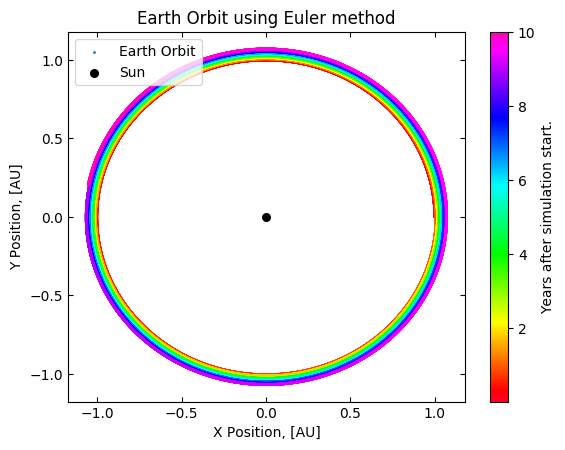
\includegraphics[width=5cm]{EarthOrbit_Euler.png}
  \caption{Earth orbit around the Sun using Eulers method}
  \label{fig:EarthOrbit_Euler}}
  \qquad
  \begin{minipage}{5cm}
    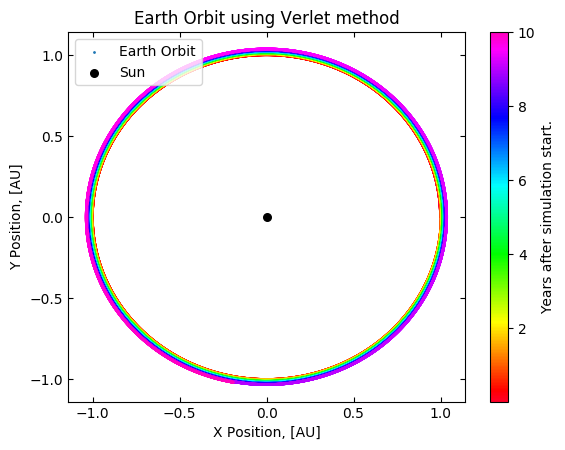
\includegraphics[width=5cm]{EarthOrbit_Verlet.png}
    \caption{Earth orbit around the Sun using Verlet's method}
    \label{fig:EarthOrbit_Verlet}
  \end{minipage}
  \end{figure}
\FloatBarrier

%skriv litt om programflow

%oppgave 5c)


\subsection{Testing}
\subsubsection{Stability with varying timestep} \label{sec:results-test-timestep}
In the figures below we plotted Earths orbit over a thousand years with different timesteps.


\begin{figure}[!h]
  \centering
  \makebox[\textwidth][c]{
  \begin{minipage}{0.7\textwidth}
        \centering
        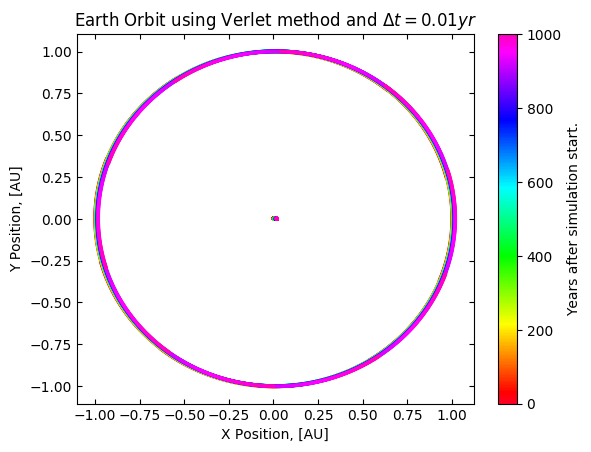
\includegraphics[width=1\textwidth]{/test/Earth-Sun_Test0-01.png} % first figure itself
    \end{minipage}\hfill
    \begin{minipage}{0.7\textwidth}
        \centering
        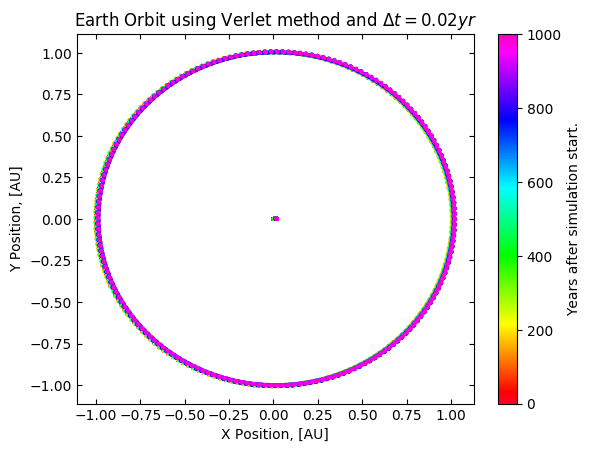
\includegraphics[width=1\textwidth]{/test/Earth-Sun_Test0-02.png} % second figure itself
    \end{minipage}
}
  \caption{Earth orbit with time steps $\Delta t = 0.01$year and $0.02$year respectively }
  \label{fig:results-Timestep1}
\end{figure}
\FloatBarrier
\begin{figure}[!h]
  \centering
  \makebox[\textwidth][c]{
  \begin{minipage}{0.7\textwidth}
        \centering
        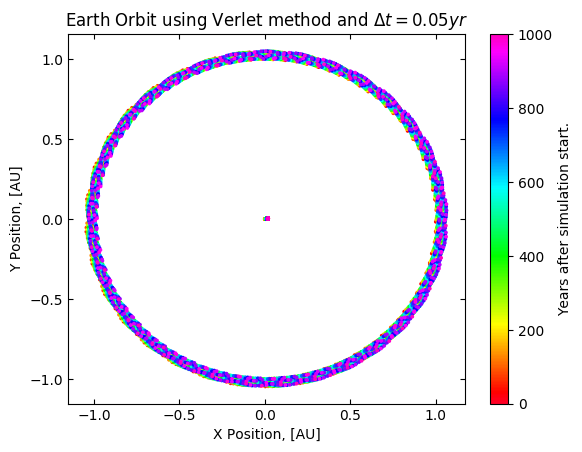
\includegraphics[width=1\textwidth]{/test/Earth-Sun_Test0-05.png} % first figure itself
    \end{minipage}\hfill
    \begin{minipage}{0.7\textwidth}
        \centering
        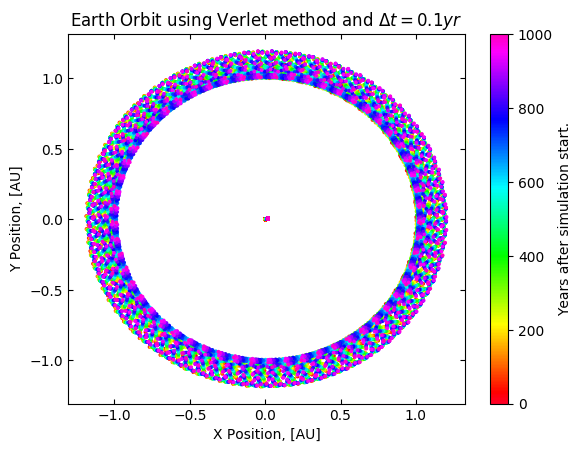
\includegraphics[width=1\textwidth]{/test/Earth-Sun_Test0-1.png} % second figure itself
    \end{minipage}
}
  \caption{Earth orbit with time steps $\Delta t = 0.05$year and $0.1$year respectively }
  \label{fig:results-Timestep2}
\end{figure}
\FloatBarrier

\subsubsection{Energy and angular momentum conservation}\label{sec:results-test-conservation}
In the figures below, kinetic energy and potential energy is plotted as a function of time in the system. We chose to simulate over a thousand years, with a timestep of $\Delta t = 0.01$.
\begin{figure}[!h]
  \centering
  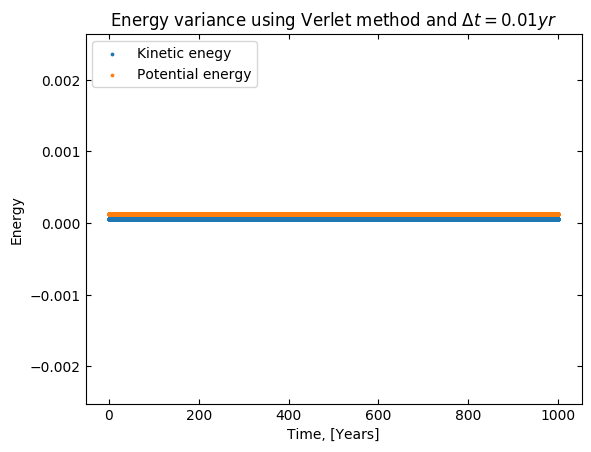
\includegraphics[width=1\textwidth]{/test/Energy_Test.png} % first figure itself
  \caption{Kinetic and Potential energy with timestep $\Delta t = 0.01$year.}
  \label{fig:results-Energies}
\end{figure}
\FloatBarrier

%oppgave 5f)
Sammenlign resultetene med de tidligere.


\end{document}
